\chapter{The Carlifornia Planet Survey Doppler Code}\label{chap:doppler}

This chapter contains a brief documentation describing the algorithm
and structure of the California Planet Survey (CPS) Doppler code,
which extracts RVs from iodine-calibrated stellar spectra. As of March
2016, no documentation in published or unpublished form existed for
this widely used code, although \cite{butler1996} describes the basics
for the technique of iodine-calibrated precise RV, and some CPS
publications contain description for certain elements of the code
\citep[e.g.,][]{2006ApJ...647..600J, 2009ApJ...696...75H, 2011ApJ...726...73H,
  2011ApJS..197...26J}.

% history of the code
Earliest documentation of code indicates 1991, co-created by Paul
Butler and Geoff Marcy. Heavily modified by John Johnson for CPS. Paul
Butler also has a version for LCPS, which he now maintains and also
serves as the pipeline for PFS and APF. Later maintained by Howard
Issacson at Berkeley. This code has been applied to data taken by
Keck/HIRES, AAT, APF, PFS, Lick/Hamilton, Magellan, HET/HRS (this
thesis), and so on. Our code is from John Johnson, version 2013.


%%%%%%%%%%%%%%%%%%%%%%%%%%%%%%%%%%%%%%%%%%%%%%%%%%%%%%%%%%%%%%%%%%%%%%%%%%%%%%
% basic algorithm, in mathematical form
\section{Basic Formulae, Algorithm, and Components}

First, we describe the basic mathematics and algorithm behind RV
extraction from iodine-calibrated stellar spectra using the CPS
code. The overall algorithm is to forward model the stellar spectra
using synthetic or empirically derived reference spectra, fitting $N$
parameters, one of which is the Doppler shift, $z$.

The reference spectra include\footnote{It can also include a model
  spectrum for a faint secondary star, telluric absorption lines (see
  Chapter~\ref{chap:keck} Section~\ref{keck:sec:telluric}), and so
  on.}: a model spectrum for the iodine absorption lines, $F_{\rm
  I_2}(\lambda)$ and a model spectrum for the star,
$F_{*}(\lambda)$. The goal is to use the model the observed,
extracted, and normalized 1-D spectrum, $F_{\rm obs}(x)$, at any given
pixel position (and spectral order), $x$, using these reference spectra
and model parameters. The broadening effect of the spectrograph is
described by the spectral response function, or the spectral point
spread function, or the instrumental profile (IP), which we will refer
to as the IP throughout this thesis and is denoted as
$\curlyp(x)$. Hence,
\beq
F_{\rm obs}(x) = \left[ F_{\rm I_2}(\lambda(x)) \times
F_{*}'(\lambda(x)) \right] \ast \curlyp(x),
\eeq
where $\lambda(x)$ is the wavelength solution for the 1-D spectrum,
and $F_{*}'$ is the red-shifted stellar spectrum defined by
$F_{*}'(\lambda) = F_{*}(\lambda\cdot(1+z))$. The Doppler shift $z$
contains two components: the stellar RV $v_*$ and the barycentric (BC)
velocity of the Earth $v_{\rm BC}$. The BC component is corrected by
$v_* = v_{\rm measured} + v_{\rm BC} + z \cdot v_{\rm BC}$.

% relative RV measurement to DSST
The stellar reference spectrum is empirically derived from iodine-free
stellar observations taken on an epoch, say, $T_0$. As a result, all
measured RVs for the star using a stellar template from $T_0$
represent relative stellar velocities between epoch $T_0$ and epoch
$T_{\rm obs}$ (i.e., $v_{*, T_{\rm obs}} - v_{*, T_0}$), instead of the
absolutely RVs of the star. The following subsection describes the
origins of the stellar (and also the iodine) reference spectra.



%----------------------------------------------------------------
% Table: RV Forward Modeling Parameters
\renewcommand{\arraystretch}{1.2} % more row spacing for the table
\begin{deluxetable}{ll}
\tabletypesize{\scriptsize}
\tablecaption{Parameters for Forward Modeling \keck\ RV Spectra\label{doppler:tab:rvpar}}
\tablewidth{320pt}
\tablehead{
  \colhead{Parameter} & \colhead{Unit and Meaning}
}
\startdata
$z$ & no unit, the stellar red shift \\
$w_0$ & \AA, wavelength of the first pixel of a spectral chunk \\
$w_d$ & \AA$/$pixel, wavelength dispersion scale for a spectral chunk \\
$A_n,\ n=1,...,12$ & no unit, amplitudes of side gaussians for IP\tablenotemark{a}
\enddata
\tablenotetext{a}{See Section~\ref{doppler:sec:ip} for more information.}
\end{deluxetable}
%----------------------------------------------------------------



% chunks
In practice, for \keck, for example, each 1-D spectrum taken at an
epoch is divided into $\sim$700 spectral chunks, each with 80 pixels
and about 2\AA\ in wavelength. One model is created and fitted for
each spectral chunk, with the model parameters listed in
Table~\ref{doppler:tab:rvpar}. Model parameter optimization is done
through least-$\chi^2$ fitting using the Levenberg-Marquardt (LM)
algorithm. Errors on the extracted 1-D spectrum is assumed to be
Poisson noise plus a 2\% additional representing potential errors in
the raw reduction. Initial guesses of the parameters come from the
solution for nearest B star $+$ iodine observation, with the exception
of the initial guess for $z$, which is set to be $v_{\rm BC}$ because
that is usually on the order of km/s and dominates the Doppler shift signal.

% re-sampling
To sample the reference spectra into the observed pixel grid, the code
first re-sample (using spline) each of them onto a grid finer than the
observation pixel grid by a factor of four (i.e., using a wavelength
dispersion of $w_d/4$). The wavelengths of this fine grid is provided
by the proposed wavelength solution parameters $w_0$ and $w_d$. Next,
it shifts the stellar reference spectrum according to the proposed
Doppler shift parameter $z$. Then it multiplies the shifted stellar
reference spectrum with the iodine reference spectrum, and then
convolves the product spectrum by the IP. Finally, it re-bins the
finely sampled model spectrum onto the observed pixel grid, which
yields the final normalized model spectrum $F_{\rm model, norm}(x)$.

% normalization
In reality, the observed spectrum used in the fitting is not
normalized (i.e. no blaze or continuum removal). To account for blaze
and stellar continuum, the codes divides the observed spectrum by the
normalized model spectrum, i.e., $F_{\rm obs}(x)/F_{\rm model,
  norm}(x)$, and then it fits a straight line $S(x)$ through the
divided spectrum (for a small 2\AA\ chunk, this linear approximation
seems sufficient). It then computes a new model spectrum by adding
this model ``continuum" on top, i.e., $F_{\rm model, final}(x) =
F_{\rm model, norm}(x) \times S(x)$. This way, the continuum component
in the observed spectral chunk is modeled by a linear function but
imposes no explicit parameters for the model.



%----------------------------------------------------------------
% Figure: Forward Modeling
\begin{figure}
%\epsscale{1.15}
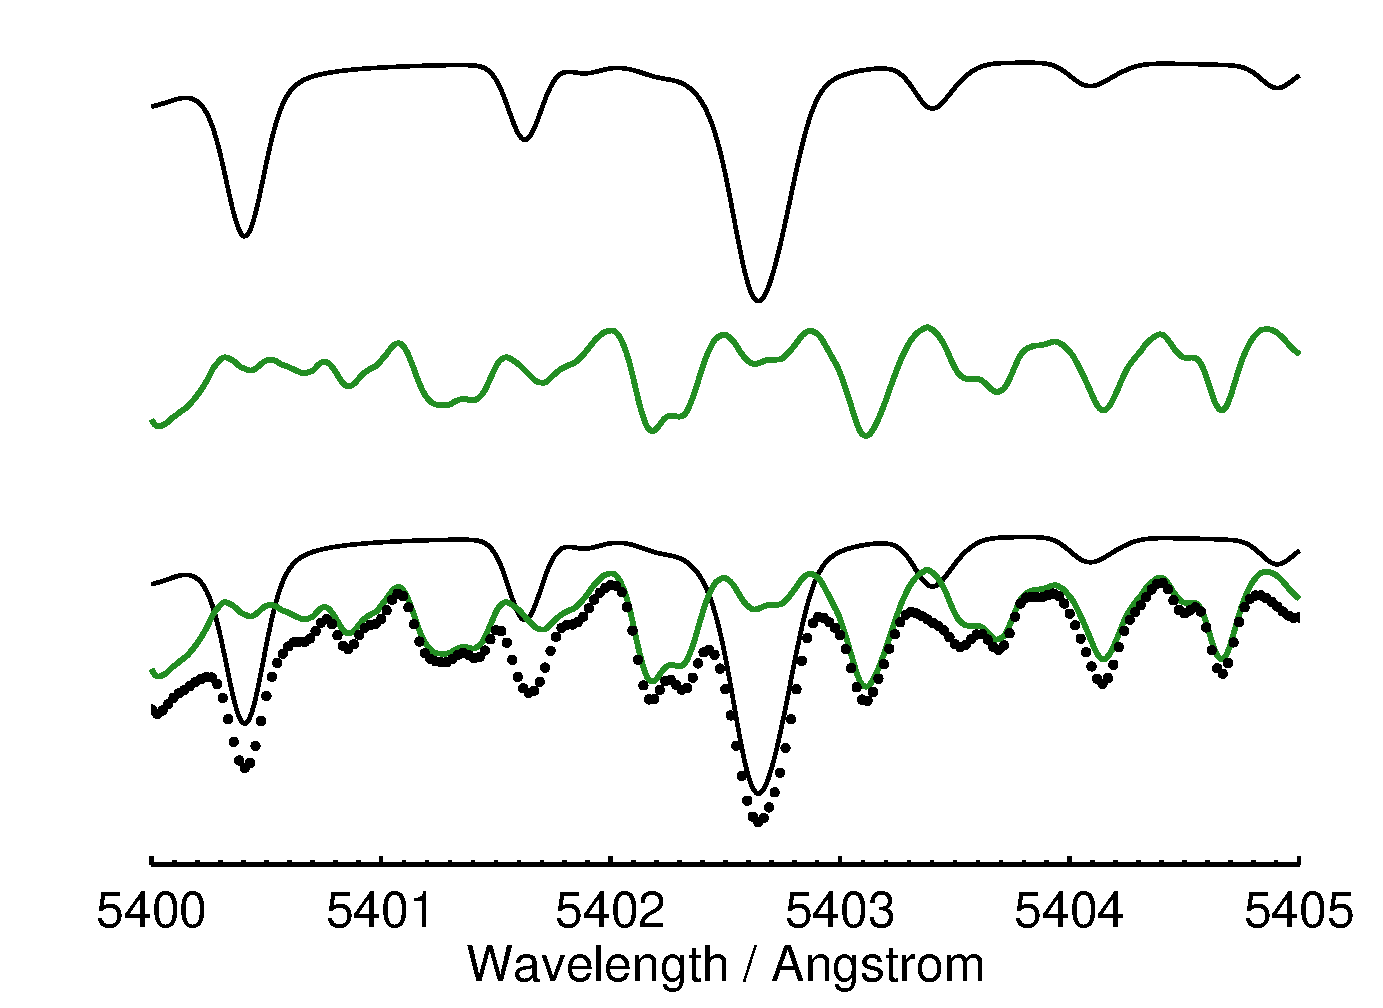
\includegraphics[scale=0.6]{doppler/forward_modeling.eps}
\caption{An illustration for the forward modeling process for
  iodine-calibrated stellar spectrum. The top black line represents
  the stellar reference spectrum (DSST), and the middle green line
  represents the iodine reference spectrum. Both reference spectra are
  convolved with an IP only for illustration purposes in order to have
  a clear match with the observed spectrum, plotted in black dots on
  the bottom. In practice, the reference spectra are multiplied {\it
    first} and then convolved with IP. \label{doppler:fig:modeling}}
\end{figure}
%----------------------------------------------------------------



%-------------------------------------------------------------------------------
\subsection{The Reference Spectra}

Ideally, the reference spectra are the ``ground truth" spectra,
i.e. the intrinsic spectra of the sources (e.g., the iodine cell, or
the star) without Doppler shift or being broadened by the
spectrometer. In reality, there is no way of knowing such ``ground
truth", so the reference spectra are empirically derived from
observations.

% how iodine atlas is made
The iodine reference spectrum, often referred to as the iodine atlas,
originates from a Fourier Transform Spectrometer scan of the iodine
cell illuminated by a continuum source. It is often of very high
signal-to-noise ratio (SNR) with high resolution (normally $\sim
500,000$ or larger). Therefore, it is generally regarded as basically
the ``ground truth" for the cell, especially for the purpose of
forward modeling lower-resolution ($\sim 60,000$) spectra. However,
there can be problems with the iodine atlas, for various reason. See
Chapter~\ref{chap:het} Section~\ref{het:sec:fts} for more on this
topic. The current FTS iodine atlas being used for \keck\ RV work is
from a scan in 1993, using the Babar FTS at NSO/KPNO, and so is the
atlas for \het. See Section~\ref{het:sec:fts} for more on iodine
reference spectra.

% how DSST is made
The stellar reference spectrum for any star, or internally to CPS
referred to as the Deconvolved Stellar Spectral Template (DSST), is
empirically derived from observed spectra of the target star. For most
of the CPS targets (bright stars), a few (4-5) observations of the
star with a narrower slit ($R \geq 80,000$) are taken without the
iodine cell in the light path. Then they are stacked together to boost
the SNR ($>500$), and then deconvolved with proper IPs derived from
bracketing B star $+$ iodine observations. The wavelength solution for
the DSST also comes from the bracketing B star $+$ iodine
observations. See Section~\ref{keck:sec:dsst} for more information and
problems related to DSSTs. For faint stars where obtaining stellar
template is expensive or unfeasible, \cite{2006ApJ...647..600J}
developed a technique where they ``morph" a synthetic stellar spectrum
or an existing DSST of another star with similar stellar properties to
fit the stellar iodine observation, and then they use this new morphed
DSST for RV extraction.


%-------------------------------------------------------------------------------
\subsection{The Functional Forms of the Instrumental Profile}\label{doppler:sec:ip}

The IP $\curlyp(x)$ can take many functional forms, and for \keck, an IP of sum of
gaussians works exceptionally well ($\chi^2 \sim 1$ for pure iodine
absorption line fit). The mathematical form for it is:
\beq
\curlyp_{\rm gaus}(x) = \sum A_n \exp{\left[\left(
    \frac{x-\mu_n}{\sigma_n} \right)^2\right]}. 
\eeq
$A_n$ stands for the amplitude for each gaussian component. $A_n$'s
are floated parameters for the fitter to optimize while $\mu_n$ and
$\sigma_n$ (i.e., positions and widths of the gaussians) have
empirically-optimized fixed values, depending on the instrument
setting of \keck\ (e.g., slit width). For \keck\ precise-RV mode (B5
decker, $\sim$60,000 resolution, with iodine cell in light path), the
IP contains 12 free parameters, $A_1, A_2, ..., A_{12}$, while $A_0$
is fixed to 1 (the big central gaussian) and $\mu_n, n=0,...,12$ and
$\sigma_n, n=0,...,12$ also have fixed values.

Another frequently used IP is the Gauss-Hermite (GH)
function, which is composed of gaussians multiplied by Hermite
polynomials $H_n$:
\beq
\curlyp_{\rm GH}(x) = \sum A_n u_n(x) = \sum A_n 
\left( \frac{2}{\pi w^2} \right)^{1/4} \frac{1}{\sqrt{n!2^2}} H_n
\left( \frac{\sqrt{2}x}{w} \right) \exp{\left[
    -\left(\frac{x}{w}\right) ^2  \right]}.
\eeq
Mathematically, any sum of gaussians can be decomposed into orthogonal
GH terms\footnote{See
  http://math.stackexchange.com/questions/28719/how-to-decompose-displaced-hermite-gauss-function-into-higher-order-hgs
  for an illustration, retrieved on March 18 2016.}, and therefore, in
principle, the GH IP should present a generic and flexible option for
IP choices. However, in reality, the least-$\chi^2$ solver is
extremely sensitive to the choices of initial guesses, even for
orthogonal bases. As a result, GH IP normally does not outperform sum
of gaussians (e.g., see work by \citealt{2013AAS...22114908V}). The GH
IP is what we use for extracting RVs from \het\ data. See
Chapter~\ref{chap:het} Section~\ref{het:sec:ip} for more.



%%%%%%%%%%%%%%%%%%%%%%%%%%%%%%%%%%%%%%%%%%%%%%%%%%%%%%%%%%%%%%%%%%%%%%%%%%%%%%
% structure of the code
\section{Code Structure and Work Flow}

This section documents the structure of the CPS Doppler code, with the
main goal to help any reader who wishes to adopt this code for their
own work. Figure~\ref{doppler:fig:flowchart} illustrates the code's
calling sequence. 


%----------------------------------------------------------------
% Figure: Code flowchart
\begin{figure}
%\epsscale{1.15}
  \centering
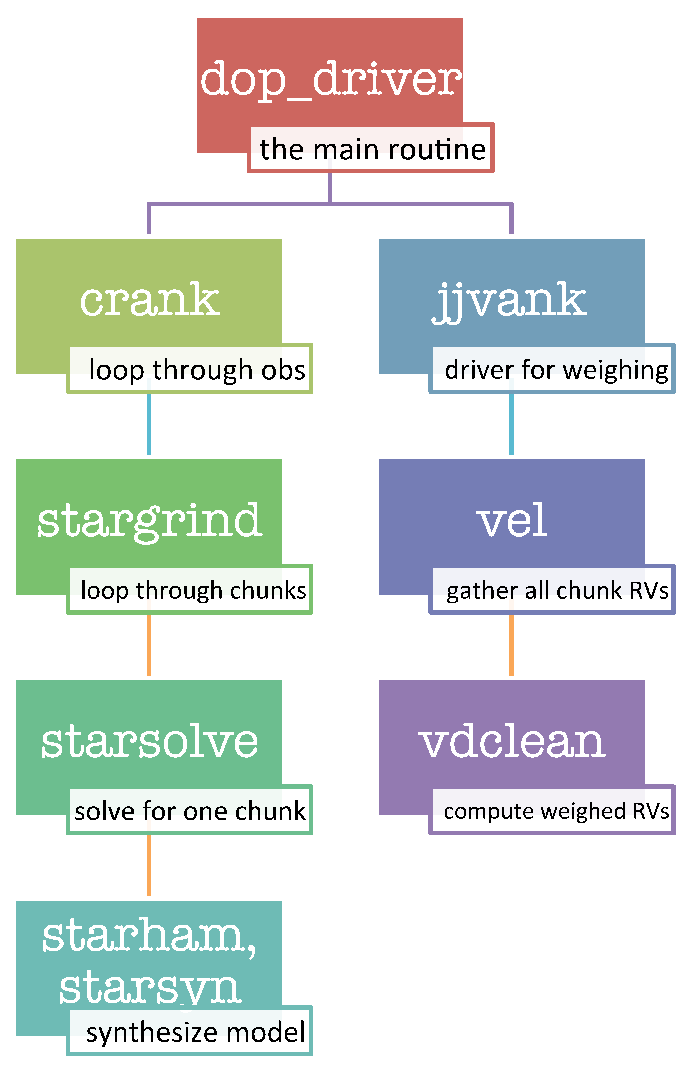
\includegraphics[scale=0.6]{doppler/flowchart.eps}
\caption{Calling sequence and main functionality for core IDL
  routines in the CPS Doppler code. \label{doppler:fig:flowchart}}
\end{figure}
%----------------------------------------------------------------


% dop_driver.pro and output files
The most top-level routine for running Doppler reduction is the IDL
procedure {\tt dop\_driver.pro}, which takes in the name of the star
and then automatically locate input files such as the extracted 1-D
spectra, the proper DSST file, the iodine atlas, and the files storing
initial guesses for parameters (which are called the {\tt vdiod}
files). The code is also very flexible with inputs and the user can
specify almost anything, e.g., a specific DSST file, choice for a
specific IP model, explicit initial guesses for parameters, and so
on. It drives the Doppler analysis and output a {\tt vd} file for each
observed spectrum, which contains best-fit parameters and other
information for all the spectral chunks. At the end, {\tt
  dop\_driver.pro} calls {\tt jjvank.pro}, which combines the RVs from
all the chunks in all the observations for this star, and evaluates
numerical weights for each chunk and each observation. Finally, {\tt
  jjvank.pro} computes the weighted RV for each observation and its RV
uncertainty and outputs the information in {\tt vst} files. The most
useful variable is the {\tt cf3} structure in the {\tt vst} file,
which contains, for example, the Julian Date (JD) of the observation
{\tt cf3.jd}, the BC {\tt cf3.bc}, the weighted RV {\tt cf3.mnvel},
and its uncertainty {tt cf3.errvel}. The algorithm for {\tt
  jjvank.pro}, or ``vanking", is described in the next
section. In the end, {\tt dop\_driver.pro} will produce $N_{\rm obs}$
{\tt vd} files and one {\tt vst} file for each star. If a new
observation is taken, a new {\tt vd} file is created, and vanking
re-evaluates the chunk and observation weights and outputs a new {\tt
  vst} file.

% crank.pro and the three passes
While {\tt dop\_driver.pro} is the routine to call for Doppler
analysis, most of its actual codes simply deal with logistical work
such as locating the right files. The real driver behind the scene is
{\tt crank.pro}, which contains the loop through all observations and
``fills out" the {\tt vd} files. In a standard CPS reduction routine,
{\tt crank.pro} is called three times. In the case of \keck\ standard
RV reduction, for example, the first time {\tt crank.pro} is called,
it fits for all 15 free parameters ($z$, $w_0$, $w_d$ and 12 IP
parameters; see Table~\ref{doppler:tab:rvpar}) for each chunk in each
observation. The LM fitter takes in the initial guesses for parameters
from B star $+$ iodine solutions and tries its best to optimize the 15-parameter
model. Due to the complexity of this multi-modal and multi-dimensional
problem, very often the best fit for this ``first pass" does not yield
a good global minimum on the $\chi^2$ surface. Therefore a second
pass of {\tt crank.pro} is called, with fixed IP parameters and thus
only three free parameters. The IP parameters are not simply fixed to last
round's best-fit values, but instead, they were fixed to describe an
``averaged" IP over a region on the CCD chip (for example, over a
neighbor of nine chunks across three spectral orders for the central
chunk). After the second pass, a third pass of {\tt crank.pro} is
called with fixed wavelength dispersion $w_d$ and only floating $z$
and $w_0$, in search for a deeper minimum or lower $\chi^2$.

% other layers inside crank.pro
Within {\tt crank.pro}, the code calls for {\tt stargrind.pro} in a
loop of all observations. {\tt stargrind.pro} does the model fitting
for a single observation, and it loops through all spectral chunks,
calling {\tt starsolve.pro}, which contains the LM fitter, for each
chunk. Inside {\tt starsolve.pro}, the spectral model is computed
using {\tt starham.pro}, which is really just a wrapper around {\tt
  starsyn.pro}. The core algorithm for model construction is all in
{\tt starsyn.pro}, which takes in the observed 1-D spectral chunk, the
DSST, the iodine atlas, and the model parameters, and outputs a model
spectrum for this chunk. 



%%%%%%%%%%%%%%%%%%%%%%%%%%%%%%%%%%%%%%%%%%%%%%%%%%%%%%%%%%%%%%%%%%%%%%%%%%%%%%
\section{Adjusting Offsets and Computing Weights for Chunk RVs}

Now all observations and all chunks have their best-fit model parameters
computed by {\tt crank.pro}, and all RVs are barycentric
corrected. What's next?

Two extremely important things need to happen at this point before we
can have an RV time series in hand, and they are accomplished by {\tt
  jjvank.pro} and most importantly, {\tt vdclean.pro} (see
Figure~\ref{doppler:fig:flowchart} for the calling sequence).

% need to adjust chunk zero point
First, the chunk RVs need to be adjusted so that they have the same
``zero point". Ideally, measured RVs from all chunks in one
observation are good estimates for the true RV of this epoch, so the
mean of all chunk RVs provides an unbiased estimate for the true RV
and their scatter provides a sense for the RV uncertainty. However, in
reality, some effects may cause the chunk RV to be biased and have a
constant offset from the true RV. One of the leading culprits is the
error in the wavelength solution of a DSST. As mentioned in the
previous section, the measured RV for each chunk at a certain epoch
$T_{\rm obs}$ is a relative RV against the DSST taken at epoch $T_0$,
$v_{*, T_{\rm obs}} - v_{*, T_0}$. This is because the stellar lines
and their Doppler shift in each chunk are modeled by red-shifting the
DSST: $F_{*}'(\lambda) = F_{*}(\lambda\cdot(1+z))$. The wavelength
solution for the DSST implies its absolute RV $v_{*, T_0}$ at
$T_0$. If the wavelength solution for all DSST chunks corresponds to
the exact same value of $v_{*, T_0}$, then measured RVs for all
chunks in the observed stellar iodine observation would have the same
``zero point". Consequently, any biases or relative errors in the DSST
wavelength solution would result in a shifted zero point for that
chunk with respect to other chunks. For example, one source of error
comes from the fact that the wavelength solution for DSST is derived
from neighboring B star $+$ iodine observations, which assumes that
the wavelength solution for the orders and pixels remain the same
between the B star and the DSST observations. Or, the wavelength
solution derived from B star observations may be imperfect. There are
also other reasons why the RV zero point of a chunk deviates from the
other chunks. Things like persisting CCD effect and certain errors in
iodine atlas or DSST can cause biases in RV estimates that contain a
constant shift component. In the end, the inconsistent RV zero points
will translate into RV scatter as we take the average of all chunk RVs
to estimate the RV for one observation. Thus, it is very important to
determine and correct for the chunk RV zero point offsets.

% need to compute weights for each chunk and observation
Second, not all spectral chunks are equal in terms of the quality of
their reported RVs, meaning that we need to take a weighted
average. There are several reasons why one chunk would consistently
have a larger RV scatter than the other. The most obvious one is
difference in the amount of Doppler information contained in the
chunks. Some chunks have more and/or deeper stellar/iodine lines,
which make them more powerful in accessing the RV information of the
star. Some chunks land on the peak of the blaze, which constantly give
them more SNR over the chunks down near the bottom. Some chunks may
contain stellar lines that have more sensitive response to stellar
activity, which would manifest as RV scatter or ``jitter". This is not
an exhaustive list, but the important thing is that there could be
many reasons which we know or do not know, and even for some of the
things we do know, we could have no way of estimate how much extra RV
scatter it would introduce to the chunk. Therefore, it is most
sensible to derive the chunk weights empirically, rather than using
any a priori ones.

% the algorithm
Overall, the algorithm for vanking works like this:


% the specifics
To be specific, most of the heavy lifting is done in {\tt vel.pro} and
{\tt vdclean.pro}. First {\tt vel.pro} calls {\tt vdcube.pro}, which
combines all {\tt vd} structures stored in the {\tt vd} files for all the
good observations. A good observation is defined by: (1) median photon
counts for all chunks is within a user-defined range; and (2) median
$\chi_\nu^2$ values of all chunks is lower than the user-defined
threshold. Otherwise {\tt vdcube.pro} will throw out the bad
observation and print out warning messages. Second, the {\tt vd} cube
put together by {\tt vdcube.pro} gets passed on to {\tt vdclean.pro},
and {\tt vdclean.pro} performs a series tasks including quality checks, outlier
rejections, RV zero point offset adjustment, and finally the
computation of chunk weights, i.e., it
\begin{enumerate}
\item Throws out chunks with bad DSST or containing no Doppler
  information (meaning it has a weight of 0 as calculated following
  the method described in \citealt{butler1996}).
\item Rejects the chunks where the fitter constantly fails to converge
  (indicated by setting $\chi_\nu^2$ to 0 or 100 in the code).  
\item Rejects the bottom 1\% (or other user-defined threshold) of the
  chunks which have the highest photon-limited RV errors (calculated
  following \citealt{butler1996}).
\item Rejects the bottom 1\% (or other user-defined threshold) of the
  chunks which have the highest $\chi_\nu^2$ values.
\item Computes the RV zero point offsets for all chunks and adjust all
  chunks to have the same zero points. Mathematically, this is done
  for each chunk by doing, say, for the i$^{\rm th}$ chunk:
  \beq
  {\rm offset_{i,j}} = \sum_{\rm j=1}^{\rm j=N_{obs}}{v_{\rm i,j}}/N
  \eeq
  where $v_{\rm i,j}$ means the reported RV for a chunk with
  index $i$ in observation $j$, and there are $N$
  observations and $M$ chunks in total, so $v_{\rm i,j}$ is a
  $M\timesN$ matrix. This is basically requiring that the mean RV
  reported by any chunk over all observations is set to zero (or any
  arbitrary value, since we only care about relative RVs across
  observations instead of the overall ``systemic" velocity of the
  star).
\item Computes chunk weights as the inverse of the estimated RV
  variance of each chunk, i.e., $1/\sigma_{\rm RV,ch}^2$. For the
  i$^{\rm th}$ chunk in the j$^{\rm th}$ observation:
  \beq
  {\rm standard\ deviation\ of\ }\left\{ \left( \Delta_{\rm ob=j,ch} \cdot
  r_{\rm ob=j} \right),\ {\rm ch=1,...,N_{ch}}\right\},
  \eeq
  where
  \beq
  \Delta_{\rm ob=j,ch=i} = v_{\rm ob=j,ch=i} - {\rm median}\left\{ v_{\rm
    ob=j,ch},\ {\rm ch=1,...,N_{ch}} \right\},
  \eeq
  and
  \beq
  r_{\rm ob=j} = {\rm median}{ \left\{ \left( |diff|/\Delta_{\rm ob=j,ch} \right),\ {\rm ch=1,...,N_{ch}} \right\} }
  \eeq
\end{enumerate} 
